% To do list for new releases: 
% - check accuracy of \currPyVersion
% 
% 

\documentclass[10pt]{article}
\setlength{\oddsidemargin}{0.in}
\setlength{\textwidth}{6.5in}
\setlength{\topmargin}{-0.25in}
\setlength{\textheight}{8.25in}

% Prevent LaTeX from adding vertical space in the middle of 
% a page just to stretch the text to match textheight
\raggedbottom

% Skip space between paragraphs
\setlength{\parskip}{.05in}

% Put numbers in section and subsection headings, but not subsubsection headings
\setcounter{secnumdepth}{2}

% Specify by how much to indent paragraphs
\setlength{\parindent}{0ex}

% Use the natbib package for the bibliography
\usepackage[round]{natbib}
\bibliographystyle{sysbio}

% Use the graphicx package to incorporate and scale
% encapsulated postscript figures
\usepackage{graphicx}
\usepackage{floatflt}

% bold math
\usepackage{bm}

% Make document single-spaced
\renewcommand{\baselinestretch}{1.0}

\usepackage{courier}	% http://www-h.eng.cam.ac.uk/help/tpl/textprocessing/fonts.html
%\usepackage{upquote}
%\newfont{\mytt}{cmtt10 at 10pt}

\newcommand{\currPhycasVersion}{1.1.2}
\newcommand{\currPyVersion}{2.6.1}

\newcommand{\trademark}[1]{#1${}^{\mbox{\tiny TM}}$}
\newcommand{\pathname}[1]{{\em #1}}				% file name or file path
\newcommand{\objectname}[1]{{\tt #1}}				% name of an object of a class (e.g. mcmc)
\newcommand{\classname}[1]{{\tt #1}}				% name of a class (e.g. MCMC)
\newcommand{\menu}[1]{{\sf #1}}					% menu command
\newcommand{\keycmd}[1]{{\sf #1}}					% keyboard command
\newcommand{\code}[1]{{\tt #1}}					% typeset using typewriter font
\newcommand{\cmd}[1]{{\tt \small #1}\index{#1}}	% phycas commands (e.g. mcmc, sumt, etc.)
\newcommand{\opt}[1]{{\tt \small #1}\index{#1}}	% command options (e.g. 'type' for model command)
\newcommand{\optval}[1]{{\tt #1}}					% option values (e.g. 'gtr' for model.type option)
\newcommand{\term}[1]{{\bfseries #1}\index{#1}}	% new term

\newcommand{\important}[1]{{\bf Important: #1}}	% important information

\newcommand{\warning}[1]{{\bf Warning: #1}}		% warnings
\newcommand{\warnNoPyThree}{\warning{Do not install Python 3.x --- Phycas is not yet ready to make the leap to Python 3}}

\newcommand{\one}[1]{\mbox{${\bf 1}_{#1}$}}
\newcommand{\data}{{\bf y}}
\newcommand{\params}{\mbox{$\bm \theta$}}
\newcommand{\Var}{\mbox{Var}}

\newcommand{\pinvar}{\mbox{$p_{\mbox{invar}}$}}
\newcommand{\ncat}{\mbox{$n_{\mbox{cat}}$}}

\newcommand{\phycasapp}{\pathname{Phycas.app}}
\newcommand{\phycasicon}{
\includegraphics[scale=0.2]{images/PhycasGUI}}

\newcommand{\Rii}[1]{-\sum_{i \neq #1} \pi_i \mu}

\newfont{\bftt}{cmtt10}

% Causes upright apostrophe (ASCII 27) to be used in verbatim rather than the 
% acute-accent-like apostrophe (ASCII 146), which causes problems when users 
% cut and paste from the manual into a Python source code file, where ASCII 146
% is not recognized
\usepackage{upquote}

% index stuff
\usepackage{makeidx}
\makeindex
%\index{cheese}			index entry
%\index{cheese!gouda} 		index subentry
%\index{cheese!gouda!brie}	index subsubentry
%\index{cheese|see{crackers}}	"see" entries
%\index{Kraft@\textit{Kraft}}	change font
%\index{cheese@gouda}		gouda right next to cheese, as if gouda were spelled cheese
\usepackage{phycas}

% Keep hyperref last among includes
\usepackage{hyperref}\hypersetup{backref, linkcolor=blue, urlcolor=blue, colorlinks=true, citecolor=blue, hyperindex=true, 
pdfstartview=FitB, 
pdfstartpage=1,
pdftitle={Phycas User Manual},
pdfauthor={Paul O. Lewis, Mark T. Holder, and David L. Swofford}, 
pdfsubject={Phycas User Manual},
pdfkeywords={phylogenetics, Bayesian, Markov chain Monte Carlo, MCMC}}
% pdfpagemode=FullScreen,  

\begin{document}

\title{{\sc Phycas User Manual} \\ Version \currPhycasVersion}
\author{Paul O. Lewis, Mark. T. Holder, and David L. Swofford}
\date{\today}
\maketitle

\tableofcontents

%%%%%%%%%%%%%%%%%%%%%%%%%%%%%%%%%%%%%%%%%%%%%%%%%%%%%%%%%%%%%%%%%%%%%%%%%%%%%%%%%%%%%%%%%%%%%%%%%%%%
%%%%% Introduction %%%%%%%%%%%%%%%%%%%%%%%%%%%%%%%%%%%%%%%%%%%%%%%%%%%%%%%%%%%%%%%%%%%%%%%%%%%%%%%%%
%%%%%%%%%%%%%%%%%%%%%%%%%%%%%%%%%%%%%%%%%%%%%%%%%%%%%%%%%%%%%%%%%%%%%%%%%%%%%%%%%%%%%%%%%%%%%%%%%%%%
\section{Introduction}

Phycas (\url{http://www.phycas.org}) is an extension of the Python programming language (\url{http://www.python.org}) that allows Python to read NEXUS-formatted data files, run Bayesian phylogenetic MCMC analyses, and summarize the results. In order to use Phycas, you need to first have Python installed on your computer. Please see section~\ref{sec:install} entitled ``Installing Phycas'' (p.~\pageref{sec:install}) for detailed installation instructions and useful information on topics important for using Phycas, such as how to obtain a command prompt for the operating system you are using. The following sections assume that you have successfully installed Phycas and have read section~\ref{sec:install}.

%%%%%%%%%%%%%%%%%%%%%%%%%%%%%%%%%%%%%%%%%%%%%%%%%%
\subsection{What's new in version 1.1.x?} %%%%%%%%
%%%%%%%%%%%%%%%%%%%%%%%%%%%%%%%%%%%%%%%%%%%%%%%%%%
These are bug-fix releases. For a description of the major bug fixed, see the section on the ``underflow'' bug in the BUGS file. For other changes, see the CHANGES file.

%%%%%%%%%%%%%%%%%%%%%%%%%%%%%%%%%%%%%%%%%%%%%%%%
\subsection{What's new in version 1.1?} %%%%%%%%
%%%%%%%%%%%%%%%%%%%%%%%%%%%%%%%%%%%%%%%%%%%%%%%%
\subsubsection{New features}
The \cmd{ps} and \cmd{sump} commands are new to version 1.1. The \cmd{ps} command allows computation of both the path sampling (a.k.a. thermodynamic integration) method of \citet{LartillotPhillippe2006} and the steppingstone sampling method introduced by \citet{XieLewisFanKuoChen2009}. See section \ref{marglike} on page \pageref{marglike} for details. The \cmd{sump} command provides an analog of the sump command in MrBayes, providing means, extremes, and credible intervals for model parameters based on samples saved in the parameter file.

\subsubsection{Bugs fixed}
Two memory leaks were fixed prior to this release. For a description of the leaks and what was done to fix them, see the section on the ``leaky'' bug in the BUGS file.

%%%%%%%%%%%%%%%%%%%%%%%%%%%%%%%%%%%%%%%%%%%
\subsection{How to use this manual} %%%%%%%
%%%%%%%%%%%%%%%%%%%%%%%%%%%%%%%%%%%%%%%%%%%
This manual begins as a tutorial by showing you how to perform a simple analysis, but does not attempt to explain all possible settings. The purpose is to quickly show you how to run the program, allowing later sections to provide detail. After the initial sections, the manual switches to reference style, detailing how to specify the model of character evolution (section~\ref{sec:models}, p.~\pageref{sec:models}) and highlighting some of the features that set Phycas apart from other Bayesian phylogenetics software (section~\ref{sec:features}, p.~\pageref{sec:features}). Toward the end you will find a discussion (in section~\ref{sec:designprinciples}) of design principles (e.g. Why did we decide to extend Python rather than write a stand-alone program? Why is there no graphical interface?) followed by an annotated listing (in section~\ref{sec:phycassettings}) of Phycas settings. The final section (\ref{sec:install}) is devoted to the details of getting Phycas (and Python) installed on your computer system.

%%%%%%%%%%%%%%%%%%%%%%%%%%%%%%%%%%%%%%%%%%%%%%%%%%%%%%%%%%%%%%%%%%%%%%%%%%%%%%%%%%%%%%%%%%%%%%%%%%%%
%%%%% Warming up to Phycas %%%%%%%%%%%%%%%%%%%%%%%%%%%%%%%%%%%%%%%%%%%%%%%%%%%%%%%%%%%%%%%%%%%%%%%%%
%%%%%%%%%%%%%%%%%%%%%%%%%%%%%%%%%%%%%%%%%%%%%%%%%%%%%%%%%%%%%%%%%%%%%%%%%%%%%%%%%%%%%%%%%%%%%%%%%%%%
\section{Warming up to Phycas} \label{sec:warmup}

Phycas is an extension of Python, so to use it you must first start Python. In this section, you will learn how to invoke Phycas commands from the Python command line. After you become familiar with the basic commands, you will probably want to create a file containing the Phycas commands for a particular analysis. Creating such a file (a Python \term{script}) makes it easier to remember exactly what analyses you performed at some later time. If you want to redo an analysis, having the commands in a script file means you do not have to type the majority of the commands over again. We will switch to using scripts in section~\ref{sec:basic} (``A basic analysis'').

%%%%%%%%%%%%%%%%%%%%%%%%%%%%%%%
\subsection{First things first}
%%%%%%%%%%%%%%%%%%%%%%%%%%%%%%% 

The way Phycas is run depends on the operating system you are using. If you are using the Windows or Linux versions, you start Phycas by opening a terminal (in Windows this is referred to as a ``console window'' or ``command prompt'') and typing \code{python} to invoke Python. If you are using a Mac, you will have downloaded the \phycasapp\ bundle that is built around the open-source terminal program iTerm (\url{http://iterm.sourceforge.net/}). Starting \phycasapp\ by double-clicking the Phycas icon automatically starts an iTerm terminal, invokes Python, and loads Phycas.

% The Phycas icon looks like this: \phycasicon

\subsubsection{Starting from a terminal on Windows}
To start Python on Windows, open a console window (a.k.a. terminal window) and type the word \code{python}. This should generate output similar to the following:
\begin{verbatim}
Python 2.5.1 (r251:54863, Oct 30 2007, 13:54:11) 
[GCC 4.1.2 20070925 (Red Hat 4.1.2-33)] on linux2
Type "help", "copyright", "credits" or "license" for more information.
>>> 
\end{verbatim}

At the \code{>>>} prompt, type \code{from phycas import *}, like this:
\begin{verbatim}
>>> from phycas import *
>>>
\end{verbatim}

Phycas is an ``extension'' of Python, but you must import extensions in order for their capabilities to be available. The import statement you typed means ``import everything phycas has to offer.'' 

\subsubsection{Starting from the \phycasapp\ bundle under MacOS}

\begin{floatingfigure}[l]{2cm}

\includegraphics[scale=0.4]{images/PhycasGUI}  
%\caption{Phycas icon}
\end{floatingfigure} If you are using the \phycasapp\ bundle on MacOS, you can launch the Phycas application by double clicking on the icon. Although the name appears to be just \pathname{Phycas}, it is really \phycasapp; the MacOS hides the \pathname{.app} extension unless you change this in the Finder preferences. (We will hereafter use the terms \term{Phycas application} and \term{Phycas.app} bundle interchangeably.) The Phycas application will show up in your dock and the window that appears will be a terminal that has already invoked Python and issued the ``from phycas import *'' command mentioned in the previous section.

All the instructions for the rest of the manual will be executed the same way regardless of whether Phycas running from a Windows console window, a Linux terminal or the \pathname{Phycas} application.

%%%%%%%%%%%%%%%%%%%%%%%%%
\subsection{Getting help}
%%%%%%%%%%%%%%%%%%%%%%%%%
Now type \cmd{help} at the Python prompt. This will display the following help message:
\begin{verbatim}
>>> help
Phycas Help
    
For Python Help use "python_help()"

Commands are invoked by following the name by () and then
hitting the RETURN key. Thus, to invoke the sumt command use:

sumt()

Commands (and almost everything else in python) are case-sensitive -- so
"Sumt" is _not_ the same thing as "sumt" In general, you should use the
lower case versions of the phycas command names.

The currently implemented Phycas commands are:
  
like                           randomtree
mcmc                           sim
model                          sump
ps                             sumt
                               

Use <command_name>.help to see the detailed help for each command. So,

sumt.help

will display the help information for the sumt command object.
\end{verbatim}

Ordinarily, typing \cmd{help} will invoke the {\em Python} help system; however, note that after Phycas has been imported into Python, typing \cmd{help} now invokes the {\em Phycas} help system. You can still access Python's interactive help by typing \cmd{python\_help()}\footnote{If you do try typing \cmd{python\_help()}, note that you can quit the Python help system (and return to using Phycas) by typing \cmd{quit} at the \code{help>} prompt}. Hopefully, the output is self-explanatory, so let's try what the output of the \cmd{help} command suggests: obtaining help for a particular command. Type the following at the Python prompt:
\begin{verbatim}
>>> model.help
model
Defines a substitution model.

Available input options:
Attribute                      Explanation
============================== =================================================
type                           Can be 'jc', 'hky' or 'gtr'

update_relrates_separately     If True, GTR relative rates will be individually
                               updated using slice sampling; if False, they will
                               be updated jointly using a Metropolis-Hastings
                               move (generally both faster and better).

relrate_prior                  The joint prior distribution for all six GTR
                               relative rate parameters. Used only if
                               update_relrates_separately is False.

relrate_param_prior            The prior distribution for individual GTR
                               relative rate parameters.  Used only if
                               update_relrates_separately is true.

relrates                       The current values for GTR relative rates. These
                               should be specified in this order: A<->C, A<->G,
                               A<->T, C<->G, C<->T, G<->T.

fix_relrates                   If True, GTR relative rates will not be modified
                               during the course of an MCMC analysis
...                               
Current model input settings:
Attribute                      Current Value
============================== =================================================
type                           'hky'
update_relrates_separately     True
relrate_prior                  Dirichlet((1.00000, 1.00000, 1.00000, 1.00000,
                               1.00000, 1.00000))
relrate_param_prior            Exponential(1.00000)
relrates                       [1.0, 4.0, 1.0, 1.0, 4.0, 1.0]
fix_relrates                   False
kappa_prior                    Exponential(1.00000)
kappa                          4.0
fix_kappa                      False
num_rates                      1
gamma_shape_prior              Exponential(1.00000)
gamma_shape                    0.5
fix_shape                      False
...
flex_prob_param_prior          Exponential(1.00000)
============================== =================================================

>>>
\end{verbatim}

You will probably need to scroll up to see all of the output of the \cmd{model.help} command. Only a portion of the output has been shown (as indicated by the ellipses). The output shows what model options are available and, at the end, the current values for those options. Thus, we see that the \opt{type} of model can be one of three things (\optval{'jc'}, \optval{'hky'} or \optval{'gtr'}) and that the current model type is \optval{'hky'}. Suppose you wanted to use the GTR model rather than the HKY model. You can do this by changing the \opt{type} option of the \cmd{model} command as follows:
\begin{verbatim}
>>> model.type = 'gtr'
>>> model.current
\end{verbatim}
Entering \code{model.current} shows the list of current values, allowing you to confirm that your change has been made.

The quotes around \optval{'gtr'} are important. They indicate to Python that you are specifying a \term{string} (a series of text characters) rather than the name of some other sort of object. If you typed \code{gtr} without the quotes, Python would assume you are referring to a variable. Because it will (presumably) not find a variable by that name, you will get the following error message if you forget the quotes:
\begin{verbatim}
>>> model.type = gtr
Error: name 'gtr' is not defined
\end{verbatim}
Note that python is forgiving about whether you use double-quotes to delimit strings or single-quotes -- either will work to tell Python that you mean a string rather than the name of a variable.
Do not be confused by the subtle differences in typesetting within this manual. In all cases you should use plain quotes in Python (not the ``back-tick'' character or any special curved quote that is found in some word-processing programs).

The option \opt{kappa\_prior} specifies the prior probability distribution to use for the transition/transversion rate ratio. Phycas defines several probability distributions for use as priors. In this case, the current value of \optval{Exponential(1.00000)} indicates that the $\kappa$ parameter will be assigned an exponential(1) prior distribution. See section~\ref{sec:probdist} (p.~\pageref{sec:probdist}) for a complete list of probability distributions available within Phycas.

The option \opt{relrates} specifies the values of the six GTR relative rates parameters. The square brackets around the value of the \opt{relrates} parameter, \optval{[1.0, 4.0, 1.0, 1.0, 4.0, 1.0]}, indicate that you should specify the six relative rate values as a Python \term{list}. The description (``The current values for GTR relative rates. These should be specified in this order: A$<$-$>$C, A$<$-$>$G, A$<$-$>$T, C$<$-$>$G, C$<$-$>$T, G$<$-$>$T.'') indicates the expected order for the six relative rate values. The \opt{relrates} option and others like it, such as \opt{kappa}, \opt{state\_freqs}, \opt{gamma\_shape}, and \opt{pinvar} are used for a variety of purposes: (1) to set the starting values for an MCMC analysis (the \cmd{mcmc} command); (2) to specify the values of parameters for simulations (the \cmd{sim} command); or (3) to specify the values of parameters for calculating the likelihood (the \cmd{like} command).

The \opt{fix\_relrates} command is used to specify whether the relative rates are to be allowed to vary during an MCMC analysis (\opt{fix\_relrates}=\optval{False}) or are to be frozen at the values specified by \opt{relrates} (\opt{fix\_relrates}=\optval{True}). The values \optval{True} and \optval{False} are known to Python and should not be surrounded by quotes (note also that case is important: typing \code{true} or \code{TRUE} will generate a ``not defined'' error message from Python).

%%%%%%%%%%%%%%%%%%%%%%%%%%%%%%%%%%%%%%%%%%%%%%%%%%%%%%%%%%%%%%%%%%%%%%%%%%%%%%%%%%%%%%%%%%%%%%%%%%%%
%%%%% A basic analysis %%%%%%%%%%%%%%%%%%%%%%%%%%%%%%%%%%%%%%%%%%%%%%%%%%%%%%%%%%%%%%%%%%%%%%%%%%%%%
%%%%%%%%%%%%%%%%%%%%%%%%%%%%%%%%%%%%%%%%%%%%%%%%%%%%%%%%%%%%%%%%%%%%%%%%%%%%%%%%%%%%%%%%%%%%%%%%%%%%
\section{A basic analysis} \label{sec:basic}

The next task is to create a Python script containing the commands to carry out a basic MCMC analysis. A Python script is a file containing Python source code (including Phycas commands). When submitted to the Python interpreter (a computer program), the commands in the script file are read and executed.  

%%%%%%%%%%%%%%%%%%%%%%%%%%%%%%%%%
\subsection{Before proceeding...}
%%%%%%%%%%%%%%%%%%%%%%%%%%%%%%%%%
Exit your current Python session by typing \keycmd{Ctrl-d} (MacOS or Linux) or \keycmd{Ctrl-z} (Windows). If you are using \phycasapp\ on MacOS, type \keycmd{Ctrl-d} one more time to exit the terminal shell (this will make the iTerm window disappear). 

Create a new, empty directory (a.k.a. folder) in which to experiment. Copy the file \pathname{green.nex} into the new directory. This file can be found under your Phycas installation directory at the location \pathname{phycas/Tests/Data/green.nex}. If you have no idea where your Phycas installation directory is located, please refer to the relevant subsection of the installation instructions (either section~\ref{subsubsec:installfolderwindows} if you are using Windows, or section~\ref{subsubsec:installfoldermac} if you are using a Mac).

%%%%%%%%%%%%%%%%%%%%%%%%%%%%%%%%%%%%%%
\subsection{The {\em basic.py} script}
%%%%%%%%%%%%%%%%%%%%%%%%%%%%%%%%%%%%%%
Create a new (plain text\footnote{It is important to save the file using plain text format. Most word processing programs, such as \trademark{Microsoft} \trademark{Word}, save files by default in a format that contains a lot of extra, proprietary information. All such programs have the option to save the file as plain text. It is best to create Python scripts using an editor that {\em only} saves files as plain text. Examples (for \trademark{Windows}) include Notepad++ and Pythonwin (or the simple Notepad program that comes with \trademark{Windows}). For Macs, Text Wrangler or BBEdit are good choices. Python comes with its own editor, named Idle, that is also a good (if slightly sluggish) choice. jEdit (\url{http://www.jedit.org/}) is a Java-Based text editor that works well on all platforms.}) file in the folder (which should contain only the file \pathname{green.nex}). Name the new file \pathname{basic.py} and type (or copy/paste) the following lines into the file:
\begin{verbatim}
from phycas import *
mcmc.data_source = 'green.nex'
mcmc.out.log = 'basic.log'
mcmc.out.log.mode = REPLACE
mcmc.out.trees.prefix = 'green'
mcmc.out.params.prefix = 'green'
mcmc.ncycles = 2000
mcmc.sample_every = 10
mcmc()
\end{verbatim}

%%%%%%%%%%%%%%%%%%%%%%%%%%%%%%%%%%%%%%%%%%%%%%%%%%%%%%%%%%%%%%%%%%%%%%%
\subsection{Line-by-line explanation} \label{subsec:basicpyexplanation}
%%%%%%%%%%%%%%%%%%%%%%%%%%%%%%%%%%%%%%%%%%%%%%%%%%%%%%%%%%%%%%%%%%%%%%%
\begin{samepage}
\begin{verbatim}
from phycas import *
\end{verbatim}
When you first start Python, it knows nothing about Phycas. You must import the functionality provided by Phycas before any of the Phycas commands described in this manual will work. This first line tells the Python interpreter to import everything (the asterisk symbol means ``everything'') from the \code{phycas} module. This line should start every Phycas script you create.\footnote{Note that you do {\em not} need to type this line if you are using the MacOS version of Phycas (although it doesn't hurt to enter \code{from phycas import *} again). The MacOS version of Phycas automatically executes this line before presenting you with the Python prompt.}
\end{samepage}

\begin{samepage}
\begin{verbatim}
mcmc.data_source = 'green.nex'
\end{verbatim}
This line specifies that the data should be read from the file named {\tt green.nex}. In our case, {\tt green.nex} is in the same directory as this script, but if it were in a different folder then you would need to specify a relative or absolute path to the file\footnote{
%
For example, if the data file was in a directory named {\tt xyz} at the same level as the directory containing the script, set \opt{data\_source} to {\tt '../xyz/green.nex'} }.
%
Phycas does not do anything at this point in the script except create a DataSource object that will read the file \code{'green.nex'} and make the \opt{mcmc.data\_source} field refer to this object. The file name is specified as a string, so surround the file name with single quotes so that the Python interpreter will not complain. 

\end{samepage}

\begin{samepage}
\begin{verbatim}
mcmc.out.log = 'basic.log'
\end{verbatim}
This line starts a log file, which captures all output sent to the console. Some consoles do not have a large buffer, and it is possible to lose the beginning of the output if an analysis runs for a long time. Note that the name of the log file must be in the form of a Python string: that is, failing to surround the file name with quotes will result in an error.
\end{samepage}

\begin{samepage}
\begin{verbatim}
mcmc.out.log.mode = REPLACE
\end{verbatim}
This line specifies the mode for the log file. The mode of any output file determines what happens if a file by that name already exists. The default behavior is to create a file by the same name but with a number at the end. For example, if \pathname{basic.log} already exists, then the new log file would be named \pathname{basic1.log}. If \pathname{basic1.log} already exists, then the new log file would be named \pathname{basic2.log}, and so on. You can also specify \code{REPLACE} (as we have done here) to replace any existing file with the same name, or \code{APPEND} to add to the end of an existing file. 
\end{samepage}

\begin{samepage}
\begin{verbatim}
mcmc.out.trees.prefix = 'green'
\end{verbatim}
This line specifies that the trees sampled during the MCMC analysis will be saved to a file having the prefix \pathname{green}. Phycas will add the extension \pathname{.t} to the end of the prefix you specify, so the full file name will be \pathname{green.t}. If you preferred, you could specify the entire file name using \code{mcmc.out.trees = 'green.t'} and \code{mcmc.out.trees.mode} could be used to specify Phycas' behavior if the file specified already exists.
\end{samepage}

\begin{samepage}
\begin{verbatim}
mcmc.out.params.prefix = 'green'
\end{verbatim}
This line specifies that the parameters sampled during the MCMC analysis will be saved to a file having the prefix \pathname{green}. Phycas will add the extension \pathname{.p} to the end of the prefix you specify, so the full file name will be \pathname{green.p}. 
\end{samepage}

\begin{samepage}
\begin{verbatim}
mcmc.ncycles = 2000
\end{verbatim}
The option \opt{ncycles} determines the length of the MCMC run. Cycles in Phycas are {\em not} the same as generations in MrBayes. About two orders of magnitude {\em fewer} Phycas cycles are needed than MrBayes generations, so a 2000 cycle Phycas run corresponds (roughly) to a 200,000 generation MrBayes run. This does not mean that Phycas runs faster (or slower) than MrBayes; it simply means that Phycas does more work during a single ``cycle'' than MrBayes does in one ``generation.''\footnote
%
{To compare the speed of MrBayes with Phycas, you should compare the time it takes, on average, to calculate the likelihood, which is the most computationally expensive task either program performs. Phycas reports this average value at the end of a run. MrBayes computes the likelihood roughly one time per generation if you specify \opt{mcmcp nrun=1 nchain=1}. Also, be sure to compare the two programs under the same model and on the same dataset and with the same computer!}
\end{samepage}

\begin{samepage}
\begin{verbatim}
mcmc.sample_every = 10
\end{verbatim}
The option \opt{sample\_every} determines how many cycles elapse before the tree and model parameters are sampled. In this case, a sample is saved every 10 cycles, so a total of 200 trees (and 200 values from each model parameter) will be saved from this run.
\end{samepage}

\begin{samepage}
\begin{verbatim}
mcmc()
\end{verbatim} 
This begins an MCMC analysis using defaults for everything except the options that you modified (\opt{data\_file\_name}, \opt{log\_file\_name}, \opt{ncycles} and \opt{sample\_every}). To see what additional settings can be changed before calling the \code{mcmc} method, either type \cmd{mcmc.help} at the Python prompt or see section~\ref{subsec:mcmcsettings} on page~\pageref{subsec:mcmcsettings}.

\subsubsection{Invoking phycas commands}
For Phycas commands such as \cmd{mcmc}, adding the parentheses after the name of the command generally serves to start the analysis that the command implements. 
There are exceptions to this rule. 
For example, the ``action'' associated with the \cmd{model} command is simply the creation of a copy of the model for purposes of saving the current model settings. 
Thus, you could issue the following command:
\begin{verbatim}
m1 = model()
\end{verbatim}
to save the current model settings to a variable named \code{m1}\footnote
%
{The name ``m1'' here is arbitrary, but you should be careful to avoid using names that are identical to those Phycas uses. For example, if you named your model ``mcmc'', then you would lose the ability to perform an MCMC analysis because you have redifined the name ``mcmc'' to mean something else!}
%
. After this point, you could make changes to \cmd{model} and conduct various analyses. 
It is unlikely that you will need to do this under ordinary circumstances (until we implement partitioned or mixture models).
We point it out only because typing \code{model()} by itself will appear to do nothing and thus might be confusing given the behavior of most Phycas commands.
Similarly the \code{randomtrees()} invocation returns a \code{TreeCollection} that holds a set of simulated trees (and does not produce visible output).
\end{samepage}

%%%%%%%%%%%%%%%%%%%%%%%%%%%%%%%%%%%%%%%%%%%%%%%%%%%%%%%%%%%%%%%%%%%%%%
\subsection{Running \pathname{basic.py}} \label{subsec:runningbasicpy}
%%%%%%%%%%%%%%%%%%%%%%%%%%%%%%%%%%%%%%%%%%%%%%%%%%%%%%%%%%%%%%%%%%%%%%

%%%%%%%%%%%%%%%%%%%%%%%%%%%%%%%%%%%%%%%%%%%
\subsubsection{If you are using Windows...} 

To execute the \pathname{basic.py} script you just created, open a console window, navigate\footnote{We suggest you read section~\ref{subsubsec:winconsole}, where a registry trick is described that enables you to open a console window positioned at a particular directory by right-clicking the name of the folder in and Explorer or My Computer window. This saves having to navigate to the directory after opening the console window, which can be a very tedious and time consuming operation if the directory in which your script resides is nested deep inside your file system.} to the directory containing the script and type the following at the command prompt:
%
\begin{verbatim}
python basic.py
\end{verbatim}

%%%%%%%%%%%%%%%%%%%%%%%%%%%%%%%%%%%%%%%%%%%
\subsubsection{If you are using MacOS...} 

Locate your \pathname{basic.py} file in a Finder window, then drag it onto the \phycasapp\ icon \phycasicon. It should start running immediately and leave you with a Python prompt \code{>>>} when it is finished. Press \keycmd{Ctrl-d} twice (once to exit Python, a second time to exit the iTerm session).

%%%%%%%%%%%%%%%%%%%%%%%%%%%%%%%%%%%%%%%%%%%
\subsubsection{Regardless of your operating system...} 

The program should run for a few minutes, creating three files (\pathname{basic.log}, \pathname{green.t} and \pathname{green.p}) as it runs. The file \pathname{green.t} is the tree file containing the trees sampled during the MCMC run, while \pathname{green.p} is the parameter file containing samples of model parameters. These files are equivalent to their counterparts in MrBayes.

%%%%%%%%%%%%%%%%%%%%%%%%%%%%%%%%%%%%%%%%%%%%%%%%%%%%%%%%%%%%%%%%%%%%%%%%%%%
\subsection{A word about pseudorandom numbers in Phycas} \label{subsec:rng}
%%%%%%%%%%%%%%%%%%%%%%%%%%%%%%%%%%%%%%%%%%%%%%%%%%%%%%%%%%%%%%%%%%%%%%%%%%%

You will notice that if you run \pathname{basic.py} twice, the results will differ slightly the second time. This is because Phycas seeds its pseudorandom number generator using the system clock, and as a result, an entirely different series of pseudorandom numbers is used for the second MCMC analysis compared to the first MCMC analysis. The results are comparable, and both are equally valid, but most of the time you would like to have the option of exactly repeating an analysis (for example, you might want to make the Phycas script used to obtain the results for a published paper available to reviewers or the scientific community). To do this in Phycas, you first create a pseudorandom number generator object, and then pass this object to all the other objects that need to generate pseudorandom numbers. The most important of these pseudorandom number clients are the \objectname{randomtree} and \objectname{mcmc} objects.

Here is a revised script (named \pathname{repeatable.py}) that does exactly what \pathname{basic.py} did, but is repeatable. It should produce exactly the same output every time it is run:
\begin{verbatim}
from phycas import *

r = ProbDist.Lot()
r.setSeed(98765)
randomtree.rng = r
mcmc.rng = r

mcmc.data_source = 'green.nex'
mcmc.out.log = 'repeatable.log'
mcmc.out.log.mode = REPLACE
mcmc.out.trees.prefix = 'green'
mcmc.out.params.prefix = 'green'
mcmc.ncycles = 2000
mcmc.sample_every = 10
mcmc()
\end{verbatim}
There are four new lines in this script. Let's go through these one by one:

\begin{samepage}
\begin{verbatim}
r = ProbDist.Lot()
\end{verbatim}
This statement creates a pseudorandom number generator object named (arbitrarily) \code{r}\footnote{The name \classname{Lot} literally means an object used to decide something by chance, as in ``casting lots''}. \classname{Lot} objects are primarily used to draw Uniform(0,1) random deviates which can be easily transformed into any other type of random variable.
\end{samepage}

\begin{samepage}
\begin{verbatim}
r.setSeed(98765)
\end{verbatim}
Before the object \code{r} is used to generate pseudorandom numbers, we must set its seed. Pseudorandom numbers (as the name suggests) are not really random, but they behave for all intents and purposes like random numbers. One difference between the numbers generated by \code{r} and real random numbers is that the former are repeatable given the same starting seed, which should be a positive integer (whole number). Here we've set the seed to the number 98765.
\end{samepage}

\begin{samepage}
\begin{verbatim}
randomtree.rng = r
\end{verbatim}
The starting tree is generated (by default) by calling \code{randomtree()}. If we want the random starting tree to be the same from run to run, we must set the \opt{rng} to \code{r}. Note that if the starting tree is different, it does not matter that we have used the same sequences of pseudorandom numbers in the MCMC analysis; we will get different results simple because we started at a different place in parameter space.
\end{samepage}

\begin{samepage}
\begin{verbatim}
mcmc.rng = r
\end{verbatim}
To force Phycas to use the same sequence of pseudorandom numbers during the MCMC analysis, set the \opt{rng} setting of \objectname{mcmc} to \code{r} as well.
\end{samepage}

%%%%%%%%%%%%%%%%%%%%%%%%%%%%%%%%%%%%%%%%%%%%%%%%%%%%%%%%%%%%%%%%%%%%%%%%%%%%%%%%%%%%%%%%%%%%%%%%%%%%
%%%%% Summarizing tree files %%%%%%%%%%%%%%%%%%%%%%%%%%%%%%%%%%%%%%%%%%%%%%%%%%%%%%%%%%%%%%%%%%%%%%%
%%%%%%%%%%%%%%%%%%%%%%%%%%%%%%%%%%%%%%%%%%%%%%%%%%%%%%%%%%%%%%%%%%%%%%%%%%%%%%%%%%%%%%%%%%%%%%%%%%%%
\section{Summarizing tree files}

Phycas provides the {\tt sumt()} method for summarizing an input tree file. While analogous, Phycas' {\tt sumt()} method differs somewhat from the MrBayes sumt command. The example below stands alone, however there is no reason why you could not place the following statements after the {\tt mcmc()} call in the previous \pathname{basic.py} example. For now, however, create a new file named \pathname{summarize.py} (in the same folder housing \pathname{basic.py}), enter the text of the example script below into the file, and save the file.

%%%%%%%%%%%%%%%%%%%%%%%%%%%
\subsection{Example script}
%%%%%%%%%%%%%%%%%%%%%%%%%%%
\begin{verbatim}
from phycas import *
sumt.trees = 'green.t'
sumt.out.trees.prefix = 'trees'
sumt.out.splits.prefix = 'splits'
sumt.burnin = 1
sumt()
\end{verbatim}

%%%%%%%%%%%%%%%%%%%%%%%%%%%%%%%%%%%%%
\subsection{Line-by-line explanation}
%%%%%%%%%%%%%%%%%%%%%%%%%%%%%%%%%%%%%
\begin{samepage}
\begin{verbatim}
from phycas import *
\end{verbatim}
These two lines were explained previously in the explanation of the \pathname{basic.py} script on page~\pageref{subsec:basicpyexplanation}. (This line would not be necessary if the \code{sumt} commands were appended to the end of \pathname{basic.py}.)
\end{samepage}

\begin{samepage}
\begin{verbatim}
sumt.trees = 'green.t'
\end{verbatim}
The setting \opt{trees} specifies the name of the tree file to be analyzed. Here, we are specifying the tree file produced by the analysis performed by \pathname{basic.py}. The file named here should be a valid NEXUS tree file, but need not be a file produced by Phycas.
\end{samepage}

\begin{samepage}
\begin{verbatim}
sumt.out.trees.prefix = 'trees'
\end{verbatim}
The setting \opt{out.trees.prefix} specifies the prefix used to create file names for a tree file (prefix + \pathname{.tre}) and a pdf file (prefix + \pathname{.pdf}). Both files will contain the same trees, but the trees in the pdf file are graphically represented whereas those in the tree file are in the form of newick (nested parentheses) tree descriptions. The first tree in each file is the 50\% majority-rule consensus tree, followed by all distinct tree topologies sampled during the course of the MCMC analysis. The graphical versions in the pdf file have edge lengths drawn proportional to their posterior means and with posterior probability support values shown above each edge. With the exception of the majority rule consensus tree, the titles of trees reflect their frequency in the samples. 
\end{samepage}

\begin{samepage}
\begin{verbatim}
sumt.out.splits.prefix = 'splits'
\end{verbatim}
The setting \opt{out.splits.prefix} specifies the prefix used to create a file name for a pdf file containing two plots. The first plot in the file is similar to an AWTY \citep[][\url{http://king2.scs.fsu.edu/CEBProjects/awty/awty_start.php}]{Nylander:2008p471} cumulative plot. It shows the split posterior probability calculated at evenly-spaced points throughout the MCMC run (as if the MCMC run were stopped and split posteriors computed at that point in the run). This kind of plot gives you information about whether the Markov chain converged with respect to split posteriors. (Often, when plots of log-likelihoods or model parameters show apparent convergence, split posteriors are still changing, making this type of plot a better indicator of convergence.) This first plot is not identical to an AWTY cumulative plot. The most striking difference is the fact that the lines plotted all originate at zero (AWTY does not plot these lines). Also, in AWTY the x-axis is labeled in terms of generations, whereas the Phycas equivalent labels the x-axis in terms of samples. 

The second plot in this file shows split sojourns. A split sojourn is a sequence of successive samples in which the split is present in the sampled tree, preceded and followed by an absense of the split. The number and duration of split sojourns gives an indication of how well the Markov chain is mixing, and this plot shows the results graphically. Neither plot in this file shows results for trivial splits (the split separating a single taxon from all other taxa; such splits are always present and are thus guaranteed to have split posterior 1.0) or for splits that were present in every sample (these are not useful from the standpoint of assessing convergence or mixing, except that poor mixing might be indicated if very few splits are plotted). See \citet{LewisLewis2005} for an example of the use of split sojourns to assess convergence. 
\end{samepage}

\begin{samepage}
\begin{verbatim}
sumt.burnin = 1
\end{verbatim}
The setting \opt{burnin} is the number of sampled tree topologies to skip. This value should always be at least 1, because the first tree in the tree file is the starting tree, which is never a valid sample from the posterior distribution. All statistics computed by the {\tt sumt()} method are based on the number of sampled trees remaining after the burn-in trees have been removed from consideration. For example, if there are 101 trees in the input tree file, and \opt{burnin} is 1, all posterior probabilities will be computed using 100 in the denominator (not 101).
\end{samepage}

\begin{samepage}
\begin{verbatim}
sumt()
\end{verbatim}
The {\tt sumt()} method call begins the analysis of the input tree file. Besides the three files produced containing trees and plots, output is generated by this method summarizing the tree topologies and splits discovered. Each summary table includes the following information:
\end{samepage}
\begin{description}
\item[freq.] The number of trees in which the split or topology was found
\item[prob.] The frequency divided by the total number of trees sampled
\item[cum] For topologies, the cumulative posterior probability over all tree topologies sorted from most to least probable. This column aids in finding credible sets of trees. For example, the 95\% credible set of tree topologies would be all those above (and including) the first one having a cumulative probability at least 0.95.
\item[weight] In the case of splits, this is the posterior mean edge length of the split, obtained by averaging the edge length associated with the split over all sampled trees in which the split was found
\item[TL] In the case of tree topologies, this is the posterior mean tree length associated with a topology, obtained by averaging the tree length associated with the topology over all sampled trees having that topology
\item[s0] This is the first sample in which the split or tree topology appeared. The minimum possible value of this quantity is 1, and the maximum is the number of trees sampled.
\item[sk] This is the last sample in which the split or tree topology appeared. The minimum possible value of this quantity is 1, and the maximum is the number of trees sampled.
\item[k] This is the number of sojourns made by the split or tree topology. A sojourn is a sequence of sampled trees in which the split or topology appears, preceded and followed by a sampled tree lacking that split or topology.
\end{description}

%%%%%%%%%%%%%%%%%%%%%%%%%%%%%%%%%%%%%%%%%%%%
\subsection{Running \pathname{summarize.py}}
%%%%%%%%%%%%%%%%%%%%%%%%%%%%%%%%%%%%%%%%%%%%
Using the same procedure outlined in section~\ref{subsec:runningbasicpy}, run your \pathname{summarize.py} script. This will produce the files \pathname{trees.tre}, \pathname{trees.pdf} and \pathname{splits.pdf}. You can open the PDF files and view or print the figures therein.

%%%%%%%%%%%%%%%%%%%%%%%%%%%%%%%%%%%%%%%%%%%%%%%%%%%%%%%%%%%%%%%%%%%%%%%%%%%%%%%%%%%%%%%%%%%%%%%%%%%%
%%%%% Probability Distributions %%%%%%%%%%%%%%%%%%%%%%%%%%%%%%%%%%%%%%%%%%%%%%%%%%%%%%%%%%%%%%%%%%%%
%%%%%%%%%%%%%%%%%%%%%%%%%%%%%%%%%%%%%%%%%%%%%%%%%%%%%%%%%%%%%%%%%%%%%%%%%%%%%%%%%%%%%%%%%%%%%%%%%%%%
\section{Probability Distributions}\label{sec:probdist}

Phycas defines several probability distributions. Several of these (Uniform, Beta, Exponential, Gamma, InverseGamma) are commonly used as prior distributions for model parameters. Others (Bernoulli, Binomial, Normal) are less commonly used as prior distributions in Bayesian phylogenetics, but are nevertheless useful for other reasons. This section briefly describes each of these distributions. 

%%%%%%%%%%%%%%%%%%%%%%%%
\subsection{Terminology}
%%%%%%%%%%%%%%%%%%%%%%%%
The \term{support} of a distribution is the set of values for which the density function is greater than zero. A distribution is a \term{discrete distribution} if the number of possible values is finite and each value is associated with a non-zero probability. Discrete distributions are associated with probability functions, $p(y|\params)$, that serve to provide the probability associated with each possible value. A distribution is a \term{continuous distribution} if the number of possible values is infinite and thus each particular value has probability zero. Continuous distributions are associated with probability density functions (\term{pdf}s). The pdf, $f(y|\params)$, provides the {\em relative} probability of each value. The pdf is scaled so that it integrates to 1.0, allowing specific {\em areas} under the pdf to be interpreted as probabilities. The \term{indicator function} \one{x=y} takes on the value 1.0 if and only if the condition in the subscript is true (i.e., $x=y$ in this example).

%%%%%%%%%%%%%%%%%%%%%%%%%%%%%%%%%%%%%%%%%%%%%%%%%%%%%%
\subsection{Using probability distributions in Phycas}
%%%%%%%%%%%%%%%%%%%%%%%%%%%%%%%%%%%%%%%%%%%%%%%%%%%%%%
In most cases, you will need to prefix the names of distributions with \code{ProbDist}. For example:
%
\begin{verbatim}
model.pinvar_prior = ProbDist.Beta(1,1)
\end{verbatim}
%
You can avoid the need for the prefix by specifically importing the distributions you need at the top of your script. For example:
%
\begin{verbatim}
from phycas.ProbDist import Beta,Gamma
...
model.pinvar_prior = Beta(1,1)
\end{verbatim}
%
Each probability distribution defined in Phycas provides a \code{sample} method that generates a single random deviate from that distribution. For example:
%
\begin{verbatim}
d = ProbDist.Gamma(0.5, 4.0)
d.sample()
11.923011659940444
\end{verbatim}
%
This can be used to get a feel for typical values generated from a distribution. To generate 10 values from a Gamma(0.5, 4.0) distribution, you can use a Python \cmd{for} loop:
%
\begin{verbatim}
d = ProbDist.Gamma(0.5, 4.0)
for i in range(10):
    d.sample()
0.21277867604109485
1.8952730436709666
0.26548236737438019
3.2718729795327026
2.5822707554839197
0.043311257125495065
0.30315706776669216
14.728064587204788
0.085634607314423447
0.10030029917676343
\end{verbatim}
%
It is also possible to get the distribution object to tell you its current mean, variance and standard deviation:
%
\begin{verbatim}
d = ProbDist.Gamma(0.5, 4.0)
d.getMean()
2.0
d.getVar()
8.0
d.getStdDev()
2.8284271247461903
\end{verbatim}
%
To set the parameters of a distribution to match a particular mean and variance, use the \code{setMeanAndVariance} method:
%
\begin{verbatim}
d = ProbDist.Normal(1.0, 1.0)
d.setMeanAndVariance(2.0, 1.0)
d.getMean()
2.0
d.getVar()
1.0
\end{verbatim}
%
To get a description of the distribution and a list of all of its methods, use the \code{help} function:
%
\begin{verbatim}
help(ProbDist.Normal)

This is a class or python type
Represents the univariate normal probability distribution.
The following public methods are available:
getMean
setLot
resetLot
getDistName
getRelativeLnPDF
getVar
lnGamma
getStdDev
clone
getLnPDF
isDiscrete
sample
setMeanAndVariance
setSeed
getCDF
\end{verbatim}
%
To get a description and usage example for a particular function, use \code{help} on the name of the function:
%
\begin{verbatim}
help(ProbDist.Exponential.setMeanAndVariance)

<unbound method Exponential.setMeanAndVariance>

An instance of type instancemethod.

Sets the mean and variance of this distribution. This distribution is
determined entirely by the mean, so the var argument is ignored. The
reason this function requires both mean and variance is for
compatibility with functions of the same name in other distributions.

>>> from phycas.ProbDist import *
>>> b = Exponential(2)
>>> print b.getMean()
0.5
>>> print b.getVar()
0.25
>>> b.setMeanAndVariance(5, 0)
>>> print b.getMean()
5.0
>>> print b.getVar()
25.0
\end{verbatim}

%%%%%%%%%%%%%%%%%%%%%%%%%%%%%%%%%%%%%%%%%%%%%%%%%%%%%%%%%%%%%%%%%%%%%%%%%%%%%%%%%%%%%%%%
\subsection{Probability distributions available in Phycas}\label{availabledistributions}
%%%%%%%%%%%%%%%%%%%%%%%%%%%%%%%%%%%%%%%%%%%%%%%%%%%%%%%%%%%%%%%%%%%%%%%%%%%%%%%%%%%%%%%%

%%%%%%%%%%%%%%%%%%%%%%%%%%%%%%%%%%%%%%%%%%%%%%%
\subsubsection{Bernoulli}\label{bernoullidist}
%%%%%%%%%%%%%%%%%%%%%%%%%%%%%%%%%%%%%%%%%%%%%%%

\renewcommand{\arraystretch}{1.5}

This distribution is provided for completeness, but currently there are no parameters in Phycas for which this distribution should be used as a prior. There are only two possible values (0 and 1), so Bernoulli distributions are appropriate for modeling stochastic processes that are characterized by presence vs. absence of something, or success vs. failure.

\begin{tabular}{lcl}
Type:                 & & Discrete \\
Parameter:            & & $p$ (probability of 1) \\
Probability function: & & $p(y|p) = p \one{y=1} + (1-p) \one{y=0}$ \\
Support:              & & $\{0,1\}$  \\
Expected value:       & & $E[y] = p$ \\
Variance:             & & $\Var(y) = p(1-p)$ 
\end{tabular}

%%%%%%%%%%%%%%%%%%%%%%%%%%%%%%%%%%%%
\subsubsection{Beta}\label{betadist}
%%%%%%%%%%%%%%%%%%%%%%%%%%%%%%%%%%%%

Beta distributions are popular as priors for parameters whose value is restricted to the interval [0.0, 1.0], such as proportions. The proportion of invariable sites parameter (often abbreviated pinvar) has a Beta prior by default in Phycas. The quantity $\Gamma(x)$ that appears in the pdf is the \term{gamma function}, which for integral values of $x$ is equal to $(x-1)!$.

\begin{tabular}{lcl}
Type:                 & & Continuous \\
Parameters:           & & $\alpha$, $\beta$   \\
Probability density function: & & $f(y|\alpha, \beta) = \frac{\Gamma(\alpha + \beta)}{\Gamma(\alpha) \; \Gamma(\beta)} \; y^{\alpha-1} \; (1-y)^{\beta - 1}$ \\
Support:              & & $[0.0,1.0]$     \\
Expected value:       & & $E[y] = \frac{\alpha}{\alpha + \beta}$ \\
Variance:             & & $\Var(y) = \frac{\alpha \beta}{(\alpha + \beta)^2 \; (\alpha + \beta + 1)}$ 
\end{tabular}

%%%%%%%%%%%%%%%%%%%%%%%%%%%%%%%%%%%%%%%%%%%%
\subsubsection{Binomial}\label{binomialdist}
%%%%%%%%%%%%%%%%%%%%%%%%%%%%%%%%%%%%%%%%%%%%

The Binomial distribution is not currently useful as a prior distribution in Phycas, and is provided for the sake of completeness. The Binomial distribution is commonly used to model counts of the number of trials satisfying some condition (a ``success''). For example, the number of heads out of 10 (independent) flips of a coin follows a Binomial distribution. The parameter of the distribution is the probability that the condition (e.g. heads) is satisfied on any given trial.

\begin{tabular}{lcl}
Type:                 & & Discrete \\
Parameters:           & & $p$ (probability of success in any given trial), $n$ (number of trials)    \\
Probability function: & & $p(y|p,n) = {n \choose y} p^y (1-p)^{n-y} $ \\
Support:              & & $\{0,1,\cdots\}$     \\
Expected value:       & & $E[y] = n p$ \\
Variance:             & & $\Var(y) = n p(1-p)$ 
\end{tabular}

%%%%%%%%%%%%%%%%%%%%%%%%%%%%%%%%%%%%%%%%%%%%%%%%%%
\subsubsection{Exponential}\label{exponentialdist}
%%%%%%%%%%%%%%%%%%%%%%%%%%%%%%%%%%%%%%%%%%%%%%%%%%

The Exponential distribution is a special case of the Gamma distribution (in which the shape parameter equals 1.0). The Exponential distribution is a common prior for parameters restricted to the positive real numbers, such as edge lengths, transition/transversion rate ratio ($\kappa$), nonsynonymous/synonymous rate ratio ($\omega$), the shape parameter of the discretized Gamma distribution used to model among-site rate heterogeneity, GTR model relative rates, and the parameters governing base frequencies.

\begin{tabular}{lcl}
Type:                 & & Continuous \\
Parameter:            & & $\lambda$ (hazard)    \\
Probability function: & & $f(y|\lambda) = \lambda e^{-\lambda y}$ \\
Support:              & & $[0.0,\infty)$     \\
Expected value:       & & $E[y] = 1/\lambda$ \\
Variance:             & & $\Var(y) = 1/\lambda^2$ 
\end{tabular}

%%%%%%%%%%%%%%%%%%%%%%%%%%%%%%%%%%%%%%
\subsubsection{Gamma}\label{gammadist}
%%%%%%%%%%%%%%%%%%%%%%%%%%%%%%%%%%%%%%

The Gamma distribution (or its special case, the Exponential distribution) is commonly used as a prior distribution for parameters defined on the positive half of the real number line. The Gamma distribution assigns probability zero for any value less than zero. Gamma distributions with shapes less than 1 have a pdf mode greater than zero. Those with shape equal to 1 are identical to Exponential distributions. In this case, the highest point reached by the pdf is $\beta$ and occurs at the value zero. If the shape is greater than 1, the pdf approaches infinity as zero is approached. The quantity $\Gamma(\alpha)$ that appears in the pdf is the \term{gamma function}, which for integral values of $\alpha$ is equal to $(\alpha-1)!$.

\begin{tabular}{lcl}
Type:                 & & Continuous \\
Parameter:            & & $\alpha$ (shape), $\beta$ (scale)    \\
Probability function: & & $f(y|\alpha,\beta) = \frac{y^{\alpha - 1} \; e^{-y/\beta}}{\beta^{\alpha} \; \Gamma(\alpha)}$ \\
Support:              & & $[0.0,\infty)$     \\
Expected value:       & & $E[y] = \alpha \beta$ \\
Variance:             & & $\Var(y) = \alpha \beta^2$ 
\end{tabular}

%%%%%%%%%%%%%%%%%%%%%%%%%%%%%%%%%%%%%%%%%%%%%%%%%%%%
\subsubsection{InverseGamma}\label{inversegammadist}
%%%%%%%%%%%%%%%%%%%%%%%%%%%%%%%%%%%%%%%%%%%%%%%%%%%%

The Inverse Gamma distribution with parameters $\alpha$ and $\beta$ is the distribution of the quantity $1/y$ if $y$ has a Gamma($\alpha,\beta$) distribution. In Phycas, the Inverse Gamma distribution is primarily used as an edge length hyperprior (see section~\ref{hierarchicalmodels} on hierarchical models). The mean of an Inverse Gamma distribution is undefined unless the shape parameter $\alpha$ is greater than 1; the variance is undefined unless $\alpha > 2$.

\begin{tabular}{lcl}
Type:                 & & Continuous \\
Parameter:            & & $\alpha$ (shape), $\beta$ (scale)    \\
Probability function: & & $f(y|\alpha,\beta) = \frac{(1/y)^{\alpha + 1} \; e^{-(1/y)/\beta}}{\beta^{\alpha} \; \Gamma(\alpha)}$ \\
Support:              & & $[0.0,\infty)$     \\
Expected value:       & & $E[y] = \frac{1}{\beta \;(\alpha-1)}$ \\
Variance:             & & $\Var(y) = \frac{1}{\beta^2 \; (\alpha-1)^2 \; (\alpha-2)}$ 
\end{tabular}

%%%%%%%%%%%%%%%%%%%%%%%%%%%%%%%%%%%%%%%%
\subsubsection{Normal}\label{normaldist}
%%%%%%%%%%%%%%%%%%%%%%%%%%%%%%%%%%%%%%%%

The normal distribution does not get a lot of use as a prior distribution because its support includes the negative real numbers, and most parameters used in Bayesian phylogenetics only make sense if they are positive.

\begin{tabular}{lcl}
Type:                 & & Continuous \\
Parameter:            & & $\mu$ (mean), $\sigma$ (standard deviation)    \\
Probability function: & & $f(y|\mu,\sigma) = \frac{1}{\sqrt{2 \pi \sigma^2}} e^{-\frac{(y-\mu)^2}{2 \sigma^2}}$ \\
Support:              & & $[-\infty,\infty)$     \\
Expected value:       & & $E[y] = \mu$ \\
Variance:             & & $\Var(y) = \sigma^2$ 
\end{tabular}

%%%%%%%%%%%%%%%%%%%%%%%%%%%%%%%%%%%%%%
\subsubsection{Uniform}\label{uniform}
%%%%%%%%%%%%%%%%%%%%%%%%%%%%%%%%%%%%%%

The Uniform distribution has been used extensively as a prior for many different continuous model parameters; however, because Uniform distributions must be truncated in order to be proper, their use as prior distributions can have some surprising effects (see \citet{Felsenstein2004} for a good discussion of the problems with truncated Uniform priors).

\begin{tabular}{lcl}
Type:                 & & Continuous \\
Parameter:            & & $a$ (lower bound), $b$ (upper bound)    \\
Probability function: & & $f(y|a,b) = \frac{1}{b-a}$ \\
Support:              & & $[a,b]$     \\
Expected value:       & & $E[y] = \frac{a + b}{2}$ \\
Variance:             & & $\Var(y) = \frac{(b - a)^2}{12}$ 
\end{tabular}

%%%%%%%%%%%%%%%%%%%%%%%%%%%%%%%%%%%%%%%%%%%%%%%%%%%%%%%%%%%%%%%%%%%%%%%%%%%%%%%%%%%%%%%%%%%%%%%%%%%%
%%%%% Models %%%%%%%%%%%%%%%%%%%%%%%%%%%%%%%%%%%%%%%%%%%%%%%%%%%%%%%%%%%%%%%%%%%%%%%%%%%%%%%%%%%%%%%
%%%%%%%%%%%%%%%%%%%%%%%%%%%%%%%%%%%%%%%%%%%%%%%%%%%%%%%%%%%%%%%%%%%%%%%%%%%%%%%%%%%%%%%%%%%%%%%%%%%%
\section{Models}\label{sec:models}

Phycas implements the standard suite of nucleotide models: JC, F81, K80, HKY, and GTR with their I, G and I+G rate heterogeneity versions. Phycas does not currently implement data partitioning, although this feature is under active development. The following sections illustrate how to set up each of the five basic classes of models listed above and how to add discrete gamma and/or proportion of invariable sites rate heterogeneity to any model.

%%%%%%%%%%%%%%%%%%%%%%%%%%%%%%%%%%%%%%%%%%
\subsection{The basic substitution models}
%%%%%%%%%%%%%%%%%%%%%%%%%%%%%%%%%%%%%%%%%%

%%%%%%%%%%%%%%%%%%
\subsubsection{JC}
%%%%%%%%%%%%%%%%%%
The JC model \citep{JukesCantor1969} constrains base frequencies and relative substitution rates to be equal.

{\bf Rate matrix}
$${\bf R} = \bordermatrix{ &     A     &     C     &     G     &   T       \cr
                         A & -3 \alpha &  \alpha   &  \alpha   &  \alpha   \cr
                         C &  \alpha   & -3 \alpha &  \alpha   &  \alpha   \cr
                         G &  \alpha   &  \alpha   & -3 \alpha &  \alpha   \cr
                         T &  \alpha   &  \alpha   &  \alpha   & -3 \alpha \cr}$$

{\bf Choosing the JC model in Phycas}
\begin{verbatim}
model.type = 'jc'
\end{verbatim}

%%%%%%%%%%%%%%%%%%%
\subsubsection{F81}
%%%%%%%%%%%%%%%%%%%

The F81 model \citep{Felsenstein1981} constrains relative substitution rates ($\mu$) to be equal but allows base frequencies ($\bm \pi$) to vary. Fixing $\pi_A = \pi_C = \pi_G = \pi_T = 0.25$ makes the F81 model equivalent to the JC model (note that $\mu = 4 \alpha$).

{\bf Rate matrix}
$${\bf R} = \bordermatrix{ &       A      &       C       &       G       &       T       \cr
                         A &    \Rii{A}   & \pi_C \; \mu  & \pi_G \; \mu  & \pi_T \; \mu  \cr
                         C & \pi_A \; \mu &    \Rii{C}    & \pi_G \; \mu  & \pi_T \; \mu  \cr
                         G & \pi_A \; \mu & \pi_C \; \mu  &    \Rii{G}    & \pi_T \; \mu  \cr
                         T & \pi_A \; \mu & \pi_C \; \mu  & \pi_G \; \mu  &     \Rii{T}   \cr}$$                                                         

{\bf Choosing the F81 model in Phycas}
\begin{verbatim}
model.type = 'hky'
model.kappa = 1.0
model.fix_kappa = True
\end{verbatim}

%%%%%%%%%%%%%%%%%%%
\subsubsection{K80}
%%%%%%%%%%%%%%%%%%%
The K80 model \citep{Kimura1980} constrains base frequencies to be equal but allows the rate of transitions to differ from the rate of transversions by a factor $\kappa = \alpha/\beta$.

{\bf Rate matrix}
$${\bf R} = \bordermatrix{ &         A          &         C          &        G          &         T          \cr
                         A & -\beta(\kappa + 2) &  \beta             &  \beta \kappa     &  \beta             \cr
                         C &  \beta             & -\beta(\kappa + 2) &  \beta            &  \beta \kappa      \cr
                         G &  \beta \kappa      &  \beta             & -\beta(\kappa + 2)&  \beta             \cr
                         T &  \beta             &  \beta \kappa      &  \beta            & -\beta(\kappa + 2) \cr}$$


{\bf Choosing the K80 model in Phycas}
\begin{verbatim}
model.type = 'hky'
model.state_freqs = [0.25, 0.25, 0.25, 0.25]
model.fix_freqs = True
\end{verbatim}

%%%%%%%%%%%%%%%%%%%
\subsubsection{HKY}
%%%%%%%%%%%%%%%%%%%
The HKY model \citep{HasegawaKishinoYano1985} allows base frequencies to be unequal and the transition/transversion rate ratio $\kappa$ to be some value other than 1.0.

{\bf Rate matrix}
$${\bf R} = \bordermatrix{ &       A      &       C       &       G       &       T       \cr
A & -\beta (\pi_Y + \pi_G \kappa) & \pi_C \; \beta  & \pi_G \; \beta \; \kappa  & \pi_T \; \beta  \cr
C & \pi_A \; \beta & -\beta (\pi_R + \pi_T \kappa) & \pi_G \; \beta  & \pi_T \; \beta \; \kappa  \cr
G & \pi_A \; \beta \; \kappa & \pi_C \; \beta  & -\beta (\pi_Y + \pi_A \kappa) & \pi_T \; \beta  \cr
T & \pi_A \; \beta & \pi_C \; \beta \; \kappa  & \pi_G \; \beta  & -\beta (\pi_R + \pi_C \kappa) \cr}$$

{\bf Choosing the HKY model in Phycas}
\begin{verbatim}
model.type = 'hky'
\end{verbatim}

%%%%%%%%%%%%%%%%%%%
\subsubsection{GTR}
%%%%%%%%%%%%%%%%%%%
The GTR model \citep{LanavePreparataSacconeSerio1984} allows base frequencies to be unequal and all six relative substitution rates ($a$, $b$, $c$, $d$, $e$ and $f$) to be different.

{\bf Rate matrix}
$${\bf R} = \bordermatrix{ &       A      &       C       &       G       &       T       \cr
A & -(\pi_C a + \pi_G b + \pi_T c) & \pi_C \; a  & \pi_G \; b  & \pi_T \; c  \cr
C & \pi_A \; a & -(\pi_A a + \pi_G d + \pi_T e) & \pi_G \; d  & \pi_T \; e  \cr
G & \pi_A \; b & \pi_C \; d  & -(\pi_A b + \pi_C d + \pi_T f) & \pi_T \; f  \cr
T & \pi_A \; c & \pi_C \; e  & \pi_G \; f  & -(\pi_A c + \pi_C e + \pi_G f) \cr}$$

{\bf Choosing the GTR model in Phycas}
\begin{verbatim}
model.type = 'gtr'
\end{verbatim}

%%%%%%%%%%%%%%%%%%%%%%%%%%%%%%%%%%%%%%
\subsection{Adding rate heterogeneity}
%%%%%%%%%%%%%%%%%%%%%%%%%%%%%%%%%%%%%%

%%%%%%%%%%%%%%%%%%%%%%%%%%%%%%%%%%%%%%%%%%%%%%
\subsubsection{Proportion of invariable-sites}
%%%%%%%%%%%%%%%%%%%%%%%%%%%%%%%%%%%%%%%%%%%%%%
A $+I$ version \citep{Reeves1992} of any of the basic substitution models means that each site is viewed as having probability $\pinvar$ of being invariable (i.e. substitution rate zero). This is one common (albeit simplistic) way to accommodate among-site rate heterogeneity in nucleotide sequence data.

\begin{verbatim}
model.pinvar_model = True
\end{verbatim}

%%%%%%%%%%%%%%%%%%%%%%%%%%%%%%
\subsubsection{Discrete gamma}
%%%%%%%%%%%%%%%%%%%%%%%%%%%%%%
A $+G$ version \citep{Yang1994} of any of the basic substitution models means that the model assumes that the distribution of rates across sites conforms to a Gamma distribution having mean 1.0. In Phycas (as in most phylogenetic software), a discretized Gamma distribution is used in practice. The number of rate categories is set using the \opt{model.num\_rates} option. If \opt{model.num\_rates} is set to any value greater than 1, the model becomes a $+G$ version.

\begin{verbatim}
model.num_rates = 4
\end{verbatim}

%%%%%%%%%%%%%%%%%%%%%%%%%%%%%%%%%%%%%%%%%%%%%%%%%%%%%%%%%%%%%%%%%%%%%%%%%%%%%%%%%%%%%%%%%%%%%%%%%%%%
%%%%% Features %%%%%%%%%%%%%%%%%%%%%%%%%%%%%%%%%%%%%%%%%%%%%%%%%%%%%%%%%%%%%%%%%%%%%%%%%%%%%%%%%%%%%
%%%%%%%%%%%%%%%%%%%%%%%%%%%%%%%%%%%%%%%%%%%%%%%%%%%%%%%%%%%%%%%%%%%%%%%%%%%%%%%%%%%%%%%%%%%%%%%%%%%%
\section{Features}\label{sec:features}

Phycas differs in some ways from other programs that conduct Bayesian phylogenetic analyses. The following sections are meant to highlight some of the features present in Phycas that are uncommon or absent in other programs.

%%%%%%%%%%%%%%%%%%%%%%%%%%%
\subsection{Slice sampling}
%%%%%%%%%%%%%%%%%%%%%%%%%%%
Phycas makes extensive use of an MCMC method known as \term{slice sampling} \citep{Neal2003a}, whereas many programs use Metropolis-Hastings (MH) proposals to update model parameters during an MCMC analysis. The decision to use slice sampling in Phycas was based on the fact that the efficiency of slice samplers can be tuned as they run. In contrast, MH depends on tuning parameters that must be adjusted prior to sampling, an activity almost never performed in practice, leading to inefficient MCMC sampling for data sets that are not like those used when decisions were being made about default values of tuning parameters. In the final tally, a program using slice sampling behaves nearly identically to one using MH if the program using MH has been tuned prior to the analysis; however, Phycas saves you from having to worry about tuning by doing it automatically during the run. 

Phycas first attempts to adapt its slice samplers (one slice sampler is assigned to each model parameter) at the cycle specified by the setting \opt{mcmc.adapt\_first}. Each subsequent adaptation occurs after twice as many cycles as the previous adaptation. After the first few adaptations there is usually little to be gained by adapting the slice samplers further, hence the increasingly long time periods between adaptations. 

Slice sampling can be used only for continuous model parameters, not for updating the tree topology. Phycas uses the \citet{LargetSimon1999} ``LOCAL move without a molecular clock'' to propose simultaneous changes in tree topology and edge lengths. Because edge length parameters are closely tied to the topology (and because there are so many of them!), it appears to be more efficient to use the LOCAL move rather than slice samplers to update edge lengths.

%%%%%%%%%%%%%%%%%%%%%%%%%%%%%%%%%%%%%%%%%%%%%%%%%%%%%%%%%%%
\subsection{Hierarchical models} \label{hierarchicalmodels}
%%%%%%%%%%%%%%%%%%%%%%%%%%%%%%%%%%%%%%%%%%%%%%%%%%%%%%%%%%%
It is common still in Bayesian phylogenetics to use non-hierarchical models. In a non-hierarchical model, all parameters in the model can be found in the likelihood function. Edge lengths are parameters found in the likelihood function and, typically, a single Exponential distribution is used as the prior distribution for all edge lengths. The problem with this is that the edge length prior often has more of an effect than intended (the average tree length often responds to changes in the edge length prior mean) and researchers are often at a loss when deciding on an appropriate prior mean for edge lengths. It is possible to take an empirical Bayes approach, which involves estimating edge lengths under maximum likelihood and using the average estimated edge length as the mean of the prior. Bayesian purists eschew this peeking at the data to help determine the prior, but how should one choose an appropriate prior distribution without using estimates? 

Phycas provides for the use of hierarchical models to solve this problem in a purely Bayesian way. In a hierarchical model, some parameters (called \term{hyperparameters}) are not found in the likelihood function. They are in this sense one level removed from the data, hence the use of the term ``hierarchical.'' In the case of edge lengths, Phycas can use a hyperparameter to determine the mean of the edge length prior distribution, taking this responsibility away from the researcher, who is relieved to learn that she now only needs to specify the parameters of the \term{hyperprior} --- the prior distribution of the hyperparameter. Because hyperparameters are one level (or more) removed from the data, the effects of arbitrary choices in the specification of the hyperprior is much less pronounced. In fact, just letting Phycas use its default hyperprior works well because it is vague enough that the hyperprior (determining edge length prior means) will begin to hover around a value appropriate for the data at hand. The effect is similar to the empirical Bayes approach, but you need not compromise any Bayesian principles and, rather than fixing the mean of the edge length prior, you are effectively estimating it as the MCMC analysis progresses.

To tell Phycas to use a hierarchical model for edge lengths, you need only set \opt{using\_hyperprior} to \code{True}. The hyperprior distribution is determined by the setting \opt{edgelen\_hyperprior}.

%%%%%%%%%%%%%%%%%%%%%%%%%%%%
\subsection{Polytomy priors}
%%%%%%%%%%%%%%%%%%%%%%%%%%%%
A solution to the ``Star Tree Paradox'' problem was proposed by \citet{LewisHolderHolsinger2005}. Their solution was to use reversible-jump MCMC to allow unresolved tree topologies to be sampled during the course of a Bayesian phylogenetic analysis in addition to fully-resolved tree topologies. If the time between speciation events is so short (or the substitution rate so low) that no substitutions occurred along a particular internal edge in the true tree, then use of the \term{polytomy prior} proposed by \citet{LewisHolderHolsinger2005} can improve inference by giving the Bayesian model a ``way out.'' That is, it is not required to find a fully resolved tree, but can drop back and punt, so to speak, by placing a lot of posterior mass on a less-than-fully-resolved topology. Please refer to the \citet{LewisHolderHolsinger2005} paper for details.

To use the polytomy prior in an analysis, be sure that \opt{allow\_polytomies} and \opt{polytomy\_prior}are both \code{True}. The setting \opt{topo\_prior\_C} determines the strength of the polytomy prior. Setting \opt{topo\_prior\_C} to 1.0 results in a flat prior (all topologies have identical prior probabilities, and thus unresolved topologies get no more or less weight than fully-resolved topologies). Setting \opt{topo\_prior\_C} greater than 1.0 favors less resolved topologies more than fully-resolved ones. This is usually what is desired; even with a prior that favors unresolved trees, a fully-resolved topology can easily win out over a less-resolved one if there is even scant evidence for substitution along the relevant edge. In the paper, this value was set to the value $e$ (the base of the natural logarithms). To do this in Phycas, set \opt{topo\_prior\_C} equal \code{math.exp(1.0)}.

The example \pathname{$<$phycas install directory$>$/phycas/Examples/Paradox/Paradox.py} shows a complete example of an analysis using the polytomy prior. If executed, this example script will recreate the analysis presented in Figure 4 of the \citet{LewisHolderHolsinger2005} paper.

%%%%%%%%%%%%%%%%%%%%%%%%%%%%%%%%%%%%%%%%%%%%%%%%%%%%%%%%%%%%%
\subsection{Marginal Likelihoods} \label{marglike} %%%%%%%%%%
%%%%%%%%%%%%%%%%%%%%%%%%%%%%%%%%%%%%%%%%%%%%%%%%%%%%%%%%%%%%%
Phycas offers several ways of estimating marginal (model) likelihoods. The marginal likelihood represents the average fit of the model to the data (as measured by the likelihood), where the average is a weighted average over all parameter values, the weights being provided by the joint prior distribution. If you initiate an MCMC analysis using the \cmd{mcmc} command, Phycas reports the marginal likelihood using the well-known harmonic mean method introduced by \citet{NewtonRaftery1994}. The {\em harmonic mean method} is widely known to overestimate the marginal likelihood, not penalizing models enough for having extra parameters that do not substantially increase the overall fit of the model. Phycas can use two alternatives to the harmonic mean method --- {\em thermodynamic integration} \citep{LartillotPhillippe2006} (also known as path sampling), and {\em steppingstone sampling} \citep{XieLewisFanKuoChen2009} --- but only if the MCMC analysis is conducted using the \cmd{ps} command. The path sampling (PS) and steppingstone sampling (SS) methods both require running a special MCMC analysis that explores a series of {\em power posterior} distributions. The power posterior is proportional to $L(\theta)^\beta p(\theta)$, where $L(\theta)$ is the likelihood, $p(\theta)$ is the prior and $\beta$ is the power. In PS or SS, $\beta$ is slowly decreased from 1 (posterior distribution) to 0 (prior distribution) in small steps. The number of $\beta$ values used is specified by \opt{ps.nbetavals} and the minimum and maximum $\beta$ values are set using \opt{ps.minbeta} and \opt{maxbeta} (it is best to leave these set to their default values of 0 and 1, respectively). \citet{XieLewisFanKuoChen2009} found that choosing $\beta$ values that are not equally spaced along the path from 1 to 0 substantially improves the efficiency of both PS and SS. Best practice appears to place most $\beta$ values close to 0. Phycas uses evenly-spaced quantiles of a Beta($a$,$b$) distribution to choose $\beta$ values, where the two shape parameters of the Beta distribution, $a$ and $b$, are specified as \opt{ps.shape1} and \opt{ps.shape2}, respectively. By default, \opt{ps.shape1} is 0.3 and \opt{ps.shape2} is 1.0. When the command \code{ps()} is invoked, an MCMC analysis is run for each of the \opt{ps.nbetavals} values of $\beta$. The current settings of the \cmd{mcmc} command are used for each value of $\beta$. The \opt{mcmc.burnin} setting governs only the initial burn-in period; there is no separate burnin between successive values of $\beta$. At the end of the run, Phycas will report the log of the marginal likelihood estimated using both the PS and SS methods.

The example \pathname{$<$phycas install directory$>$/phycas/Examples/Steppingstone/Steppingstone.py} shows a complete example of the use of path/steppingstone sampling for marginal likelihood estimation. This example recreates part of Figure 10 in the \citet{XieLewisFanKuoChen2009} paper.

%%%%%%%%%%%%%%%%%%%%%%%%%%%%%%%%%%%%%%%%%%%%%%%%%%%%%%%%%%%%%%%%%%%%%%%%%%%%%%%%%%%%%%%%%%%%%%%%%%%%
%%%%% Design principles %%%%%%%%%%%%%%%%%%%%%%%%%%%%%%%%%%%%%%%%%%%%%%%%%%%%%%%%%%%%%%%%%%%%%%%%%%%%
%%%%%%%%%%%%%%%%%%%%%%%%%%%%%%%%%%%%%%%%%%%%%%%%%%%%%%%%%%%%%%%%%%%%%%%%%%%%%%%%%%%%%%%%%%%%%%%%%%%%
\section{Design principles}\label{sec:designprinciples}

The design principles underlying Phycas are presented best as a series of questions and answers.

%%%%%%%%%%%%%%%%%%%%%%%%%%%%%%%%%%%%%%%%%%%%%%%%%%%%%%%%%%%%%%
\subsection{Why was Phycas written as an extension to Python?}
%%%%%%%%%%%%%%%%%%%%%%%%%%%%%%%%%%%%%%%%%%%%%%%%%%%%%%%%%%%%%%
\index{why Python?}Most phylogenetic analyses take a considerable amount of time to run, and thus most phylogenetic analysis software provides a mechanism for batch processing. 
Batch processing is ordinarily accomplished through the use of a command syntax of some sort that allows the user to specify the sequence of commands to run. For example, PAUP* allows PAUP blocks to be placed in NEXUS files. The user can run an analysis without manual intervention by simply executing such a file containing PAUP* commands. 
This mode has the added benefit of creating a record of exactly the analysis performed, so that later on when the reviews come back and you are trying to respond to reviewers' concerns, you can actually recall what you did! 
Using menu-driven programs makes this difficult unless the software saves a history of all keystrokes and menu selections. 
Other popular programs have their own, private command languages. 
For example, MrBayes uses MRBAYES blocks in NEXUS files, Hy-Phy uses a C-like language, and Beast uses xml as its medium for communicating commands. The problem (as we see it) with all of these is that the language used to communicate with the program is: (1) proprietary, (2) unique, and (3) incomplete. 
The proprietary and unique nature of these languages means you have only the documentation provided by the program's authors to guide you. 
Once that is exhausted, you must resort to emailing the authors, who are often so swamped with requests for information that they can only respond to a small fraction of requests. 
The incomplete nature of these languages means that many things one would like to do are not possible. 
The reason we chose to extent Python is so that we could use an existing, well-documented, widely-available computing language as the command language for Phycas. 
There are many books available on using Python, which means we do not have to provide all the details, and Python is a very powerful computing language, meaning you can write very sophisticated scripts that do anything your heart desires in your phylogenetic analysis. 
With the phylogenetic library of tools supplied by Phycas, you can even invent new phylogenetic methods if you are so inclined. 
There is, of course, some program-specific learning you must do in order to use Phycas; just having a prior knowledge of Python will not save you from reading this manual to learn what Phycas offers and how to access those features.
We feel, however, that using a powerful, existing computing language to communicate with Phycas instead of ``rolling our own'' program-specific language was a very good idea.

%%%%%%%%%%%%%%%%%%%%%%%%%%%%%%%%%%%%%%%%%%%%%%%%%%%%%%%%%%%%
\subsection{Why is there no graphical user interface (GUI)?}
%%%%%%%%%%%%%%%%%%%%%%%%%%%%%%%%%%%%%%%%%%%%%%%%%%%%%%%%%%%%
\index{graphical user interface}Due to the large scale at which DNA sequencing is performed these days, and the increasing desire to ``pipeline'' analyses, we felt that using a script-based approach would best serve the needs of potential users in the near and distant future. Python is already installed on most unix-based operating systems (including Linux and MacIntosh OSX), and thus Phycas can be easily inserted in to bioinformatics pipeline applications. Although it does not come pre-installed on new systems, Python is easy to install on \trademark{Windows}-based PCs, and thus Phycas can be used easily on any workstation or laptop. While many users like user-friendly GUIs with pull-down menus and dialog boxes, software that depends on a GUI has certain disadvantages: (1) cannot be pipelined easily; (2) cannot be run on a remote cluster; and (3) often does not allow one to save a record of the exact analysis performed. One of the strong benefits of a GUI is that it allows experimentation and visualization. Phycas provides for visualization by outputting trees and plots in the form of PDF files. While not quite as appealing as an on-screen visual representation, PDF files provide what most of us really need: the ability to insert a publication-quality figure into a manuscript, or load artwork into other programs for manipulation.  

%%%%%%%%%%%%%%%%%%%%%%%%%%%%%%%%%%%%%%%%%%%
\subsection{Is Phycas slower than MrBayes?}
%%%%%%%%%%%%%%%%%%%%%%%%%%%%%%%%%%%%%%%%%%%
All scripting-based languages (R, Python, Perl, Ruby) are relatively slow compared to compiled languages such as C and C++. Fortunately, the Boost Python library (\url{http://www.boost.org/libs/python/doc/}) has made it easy to write the parts of Phycas that need to be fast in C++ and export these routines so that they can be called from Python. As a result, Phycas competes favorably with any phylogenetic software application out there in terms of speed. If you make speed comparisons of Phycas to other programs, be sure to compare them in a fair way. Phycas uses a different definition of ``generation'' than does MrBayes, for example. Because a ``cycle'' in Phycas is equivalent to more than 100 ``generations'' in MrBayes, it is easy to conclude that Phycas is slow compared to MrBayes. To be fair, compare instead the time required for some (large) number likelihood calculations under comparable models. Phycas makes this easy by reporting the number of likelihood calculations performed and the time required at the end of an MCMC analysis\index{comparing speed}.

%%%%%%%%%%%%%%%%%%%%%%%%%%%%%%%%%%%%%%%%%%%%%%%%%%%%%%%%%%%%%%%%%%%%%%%%%%%%%%%%%%%%%%%%%%%%%%%%%%%%
%%%%% Settings %%%%%%%%%%%%%%%%%%%%%%%%%%%%%%%%%%%%%%%%%%%%%%%%%%%%%%%%%%%%%%%%%%%%%%%%%%%%%%%%%%%%%
%%%%%%%%%%%%%%%%%%%%%%%%%%%%%%%%%%%%%%%%%%%%%%%%%%%%%%%%%%%%%%%%%%%%%%%%%%%%%%%%%%%%%%%%%%%%%%%%%%%%
\section{Settings}\label{sec:phycassettings}
This section lists all currently available Phycas settings. 
You will find more if you look at the \code{Phycas.\_\_init\_\_} method in the \pathname{Phycas.py} file, but be forewarned that settings found in \pathname{Phycas.py} but not listed here are experimental and not fully tested --- use at your own risk.
Please do not ask for help with undocumented settings: we will document them here when we feel they are ready to be used.

\subsection{Settings used by \code{like}}\label{subsec:likesettings}
\input{like}
\subsection{Settings used by \code{mcmc}}\label{subsec:mcmcsettings}
\input{mcmc}
\subsection{Settings used by \code{model}}\label{subsec:modelsettings}
\input{model}
\subsection{Settings used by \code{randomtree}}\label{subsec:randomtreesettings}
\input{randomtree}
\subsection{Settings used by \code{ss}}\label{subsec:sssettings}
\paragraph[Input options]{Input options:}\begin{description}
\item[\bftt  nbetavals] The number of values beta will take on during the run; for example, if this value is 4, then beta will take on these values: 1, 2/3, 1/3, 0 (default: {\bftt  101})
\item[\bftt  ti] If True, the marginal likelihood will be estimated using thermodynamic integration and the stepping stone method with reference distribution equal to the prior; if False (the default), the stepping stone method with reference distribution approximating the posterior will be used (this greatly improves the accuracy of the stepping stone method and is strongly recommended). (default: {\bftt  False})
\item[\bftt  xcycles] The number of extra cycles (above and beyond mcmc.ncycles) that will be spent exploring the posterior (additional posterior cycles help stepping stone analyses formulate an effective reference distribution). (default: {\bftt  0})
\item[\bftt  maxbeta] The first beta value that will be sampled. (default: {\bftt  1.0})
\item[\bftt  minbeta] The last beta value that will be sampled. (default: {\bftt  0.0})
\item[\bftt  minsample] Minimum sample size needed to create a split-specific edge length working prior. (default: {\bftt  10})
\item[\bftt  shape1] The first shape parameter of the distribution used to determine the beta values to be sampled. This distribution is, confusingly, a Beta distribution. Thus, if both shape1 and shape2 are set to 1, beta values will be chosen at uniform intervals from minbeta to maxbeta. (default: {\bftt  1.0})
\item[\bftt  shape2] The second shape parameter of the distribution used to determine the beta values to be sampled. This distribution is, confusingly, a Beta distribution. Thus, if both shape1 and shape2 are set to 1, beta values will be chosen at uniform intervals from minbeta to maxbeta. (default: {\bftt  1.0})
\end{description}

\subsection{Settings used by \code{sump}}\label{subsec:sumpsettings}
\input{sump}
\subsection{Settings used by \code{sumt}}\label{subsec:sumtsettings}
\input{sumt}

%%%%%%%%%%%%%%%%%%%%%%%%%%%%%%%%%%%%%%%%%%%%%%%%%%%%%%%%%%%%%%%%%%%%%%%%%%%%%%%%%%%%%%%%%%%%%%%%%%%%
%%%%% Installing Phycas %%%%%%%%%%%%%%%%%%%%%%%%%%%%%%%%%%%%%%%%%%%%%%%%%%%%%%%%%%%%%%%%%%%%%%%%%%%%
%%%%%%%%%%%%%%%%%%%%%%%%%%%%%%%%%%%%%%%%%%%%%%%%%%%%%%%%%%%%%%%%%%%%%%%%%%%%%%%%%%%%%%%%%%%%%%%%%%%%
\section{Installing Phycas}\label{sec:install}

%%%%%%%%%%%%%%%%%%%%%%%%%%%%%%%%%%%%%%%%%%%%%%%%%%%%%%%
\subsection{Instructions for \trademark{Windows} users} 
%%%%%%%%%%%%%%%%%%%%%%%%%%%%%%%%%%%%%%%%%%%%%%%%%%%%%%%

These instructions assume you are using \trademark{Windows} \trademark{XP} or \trademark{Vista}.

\subsubsection{\trademark{Windows} console} \label{subsubsec:winconsole}

One very handy feature that does not come with \trademark{Windows} is the ability to open a command console by using the right-click speed menu in \trademark{Explorer}. The web site \url{http://www.commandline.co.uk/cmdhere/} describes how to add this functionality, which will make Phycas {\em much} easier to use (it is not required, however, in order to use Phycas). The basic procedure is to create a file named \pathname{cmdhere.reg} with the following text (or download the file from the web site above):
%
\begin{verbatim}
REGEDIT4

[HKEY_CLASSES_ROOT\*\shell\cmdhere]
@="Cmd&Here"

[HKEY_CLASSES_ROOT\*\shell\cmdhere\command]
@="cmd.exe /c start cmd.exe /k pushd \"%L\\..\""

[HKEY_CLASSES_ROOT\Folder\shell\cmdhere]
@="Cmd&Here"

[HKEY_CLASSES_ROOT\Folder\shell\cmdhere\command]
@="cmd.exe /c start cmd.exe /k pushd \"%L\""
\end{verbatim}
%
Assuming that you saved this file with the extension \pathname{.reg}, the \trademark{Windows} operating system will know what to do with it. Double-click the name of the file in \trademark{Windows} \trademark{Explorer}, and the required registry entry will be made. \warning{making changes to your system's registry is a bit risky, and we take no responsibility for any damage your system may incur by following these directions!} That said, this worked fine for us and saves an enormous amount of time. \trademark{Windows} offers a PowerToy (\url{http://www.microsoft.com/windowsxp/downloads/powertoys/xppowertoys.mspx}) for \trademark{XP} that does something similar. While perhaps safer to install, it is somewhat frustrating to use because if you are already inside a directory in which you want to open a console, you must first go up one level in order to open a console window for that directory.

\subsubsection{Installing Python under \trademark{Windows}}

Before you go to the trouble of downloading and installing Python, make sure you do not already have Python installed on your Windows system. From the Start button, choose \menu{All Programs}, then \menu{Accessories} and finally \menu{Command Prompt}. Type \code{python -V} in the console window that appears, and if a phrase such as \code{Python 2.5.1} appears, then you already have Python installed! Most Windows users will probably see \code{'python' is not recognized as an internal or external command, operable program or batch file.} In this case, you need to visit \url{http://python.org} and download and install the latest version of Python (version \currPyVersion\ as of this writing). \warnNoPyThree

\subsubsection{Installing Phycas under \trademark{Windows}}

Visit the Download section of the Phycas web site \url{http://phycas.org/} and download the Windows installer. If you are using Windows XP, double-click the installer to install Phycas. If using Vista, right-click the installer and choose to install as Administrator. The installer will attempt to identify the location of Python on your system, and if it fails to find Python will abort the installation. Assuming it can find Python, it will install Phycas into the \pathname{Lib/site-packages} directory of that Python installation. 

\subsubsection{Locating the ``Phycas Installation Folder'' under \trademark{Windows}} \label{subsubsec:installfolderwindows}

You will find a Phycas section in the menu that appears when you choose \menu{Start} and \menu{All Programs}. Included in the \menu{Start/All Programs/Phycas} menu is an item named \menu{Phycas Installation Folder}. Choosing this menu item will open \trademark{Windows} (file) Explorer to the ``Phycas Installation Folder'' mentioned in the tutorial.

%%%%%%%%%%%%%%%%%%%%%%%%%%%%%%%%%%%%%%%%%%%%%
\subsection{Instructions for MacIntosh Users}
%%%%%%%%%%%%%%%%%%%%%%%%%%%%%%%%%%%%%%%%%%%%%

These instructions assume you are using MacOS 10.4 or later.

\subsubsection{The iTerm terminal application}

Bundled with Phycas is a terminal application called iTerm. The iTerm application is an open-source replacement for the Terminal application with which you may be familiar (and which comes with the MacOS). While it is possible to use Phycas from Terminal, we recommend strongly that you use the iTerm application that comes with Phycas. The iTerm application starts automatically when you click on the icon labeled ``Phycas'' (see below) or drop a script file onto the icon. The main reason for using the bundled iTerm application is that it starts Python and imports phycas for you automatically when it is started.

\subsubsection{Installing Python on a Mac}

If you are using MacOS 10.4, and haven't installed Python yourself, your Mac probably has Python 2.3 installed. To find out, open a terminal window (you can find the Terminal app in the Utilities folder, which is itself a subfolder of the \pathname{Applications} folder) and type \code{python -V}. If the version of Python is 2.3, you will need to visit \url{http://python.org} and download and install the latest version of Python (version \currPyVersion\ as of this writing). \warnNoPyThree

\subsubsection{Installing Phycas on a Mac}

Visit the Download section of the Phycas web site \url{http://phycas.org/} and download the MacOS DMG file. Once the DMG file has been downloaded, double-click it to mount it. Inside the DMG, you should find several files (Figure~\ref{phycasdmg}). Copy the ``file'' named \pathname{Phycas} (which is actually a special ``application bundle'' folder named \phycasapp, but the operating system hides the \pathname{.app} part of the name) to your \pathname{Applications} folder and the file named \pathname{manual.pdf} to a folder of your choice. To start Phycas, double-click the \phycasapp\ application or, alternatively, drop a script file with Phycas commands onto it. \important{When you start Phycas, you are actually starting an application named iTerm that has been bundled with the Phycas Python libraries. Thus, the menu items you see are iTerm menu items (including the \menu{Update...} menu item)}. With this MacOS version, you need not type the \code{from phycas import *} command because this is done for you when you double-click \phycasapp.

\subsubsection{Locating the ``Phycas Installation Folder'' on a Mac} \label{subsubsec:installfoldermac}

The ``Phycas Installation Folder'' that is mentioned in the tutorial is inside the \phycasapp\ application bundle. MacOS tries to make it difficult for you to see inside application bundles, but clicking on the \phycasapp\ bundle while pressing the \keycmd{Ctrl} will produce a menu, and choosing the \menu{Show Package Contents} item on that menu will allow you to view the contents of the application bundle folder. Once inside \phycasapp, double-click on the \pathname{Contents} folder, then the \pathname{Resources} folder to find the Phycas Installation folder, which is simply named \path{phycas}.

%
% Figure "phycasdmg"
%
\begin{figure}[t]
\begin{center}
\begin{minipage}{5.in}
\hfil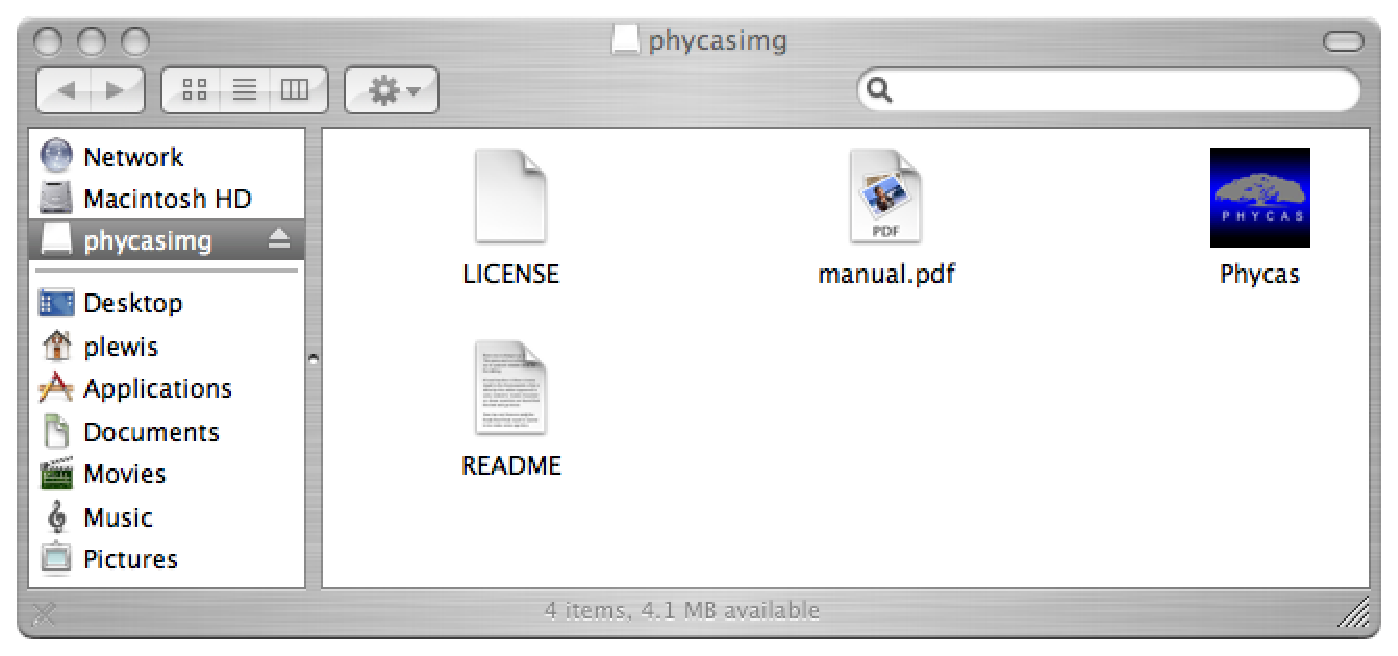
\includegraphics[scale=0.5]{images/phycasdmg}\hfil
\caption{\small The Phycas DMG file after it has been mounted.}
\label{phycasdmg}
\end{minipage}
\end{center}
\end{figure}

%%%%%%%%%%%%%%%%%%%%%%%%%%%%%%%%%%%%%%%%%%%%%%%%%%%%%%%%%%%%%%%%%%%%%%%%%%%%%%%%%%%%%%%%%%%%%%%%%%%%
%%%%% References %%%%%%%%%%%%%%%%%%%%%%%%%%%%%%%%%%%%%%%%%%%%%%%%%%%%%%%%%%%%%%%%%%%%%%%%%%%%%%%%%%%
%%%%%%%%%%%%%%%%%%%%%%%%%%%%%%%%%%%%%%%%%%%%%%%%%%%%%%%%%%%%%%%%%%%%%%%%%%%%%%%%%%%%%%%%%%%%%%%%%%%%
\section*{References}\addcontentsline{toc}{section}{References}
\renewcommand{\bibsection}{}
\bibliography{manual}

\printindex

\end{document}
